% Created 2017-11-01 mer. 15:55
\documentclass[11pt]{article}
\usepackage[utf8]{inputenc}
\usepackage[T1]{fontenc}
\usepackage{fixltx2e}
\usepackage{graphicx}
\usepackage{longtable}
\usepackage{float}
\usepackage{wrapfig}
\usepackage{rotating}
\usepackage[normalem]{ulem}
\usepackage{amsmath}
\usepackage{textcomp}
\usepackage{marvosym}
\usepackage{wasysym}
\usepackage{amssymb}
\usepackage{hyperref}
\tolerance=1000
\usepackage {algorithm}
\author{Mathieu Mandret}
\date{\today}
\title{Algorithmes génétiques: application au problème du voyageur de commerce.}
\hypersetup{
  pdfkeywords={},
  pdfsubject={},
  pdfcreator={Emacs 25.3.1 (Org mode 8.2.10)}}
\begin{document}

\maketitle
\tableofcontents


\section{Le problème du voyageur de commerce}
\label{sec-1}
On cherche à determiner quel est l'ordre de parcours optimal de $n$ villes. Ici, nous considérons que la ville de départ est un critère determinant,
donc $A \rightarrow B \rightarrow C  \neq   C \rightarrow A \rightarrow B$ même si l'ordre des villes à l'intérieur du 
voyage reste le même. On est ici face à un problème d'explosion combinatoire, la liste des parcours est en fait la liste des permutations des villes.
Par exemple, pour 3 villes $A, B \text{et } C$ on a les possibilités suivantes:
$A B C \\ A C B \\ B A C \\ B C A \\ C A B \\ C B A$

Pour $n$ villes, on a $n!$ permutations. La fonction factorielle croît extrement rapidement avec $n$.
\begin{figure}[htb]
\centering
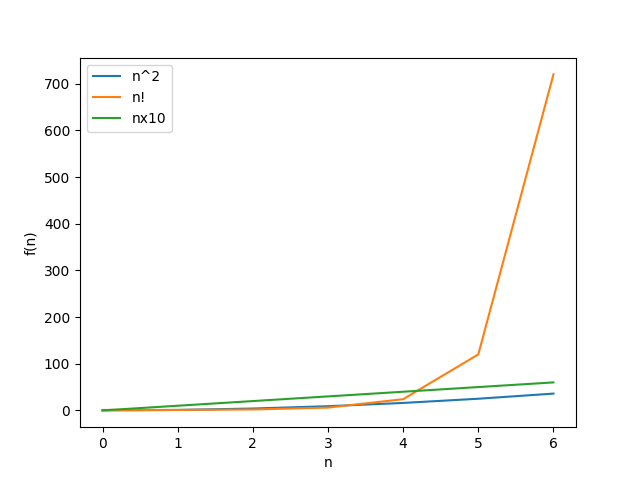
\includegraphics[width=.9\linewidth]{./complexite.png}
\caption{Croissance de la fonction factorielle comparée à $n^2$ et $n\times10$}
\end{figure}

Il est encore envisageable d'énumerer toutes ces permutations pour des $n$ relativement petits comme $10! = 3628800$ mais $30! = 265252859812191058636308480000000$ il n'est plus possible
de calculer toutes les permutations dans un temps raisonnable. On ne peut donc pas proposer d'algorithme deterministe pour résoudre le problème du voyageur de commerce dès que le nombre de villes
dépasse 10. La solution est d'utiliser un \textbf{algorithme génétique}. Il sera implémenté dans la langage
Python dans sa version 3.6 en utilisant les librairies \emph{math}, \emph{matplotlib} et \emph{numpy}

\section{L'algorithme génétique}
\label{sec-2}
Avant d'expliquer l'algorithme en lui même, il est important de déterminer la représentation informatisée du problème du voyageur de commerce.
On utilisera un paradigme de programmation orienté objet, ou les classes seront: Ville, Chemin et Population.
\subsection{Les villes}
\label{sec-2-1}
Une ville est représentée par une un couple de flottants correspondants à ses coordonées $(X,Y)$. Un exemple d'instanciation d'une ville en $X = 1$ et $Y = 5$ serait:
\begin{verbatim}
v1 = Ville(1, 5)
\end{verbatim}
Pour calculer la longueur d'un chemin, il faut déjà pouvoir determiner la distance d'une ville à une autre
la classe ville implemente donc la méthode \emph{distance$_{\text{to}}$} dont l'en-tête est:
\begin{verbatim}
def distance_to(self, other)
\end{verbatim}

Le paramètre \emph{self} fait réference a la ville courante et other à l'autre ville. Elle retourne la distance entre
les coordonnées de chaque ville calculée grâce à la formule:
$\text{distance} = \sqrt{(X_a-X_b)^2+(Y_a-Y_b)^2}$
Cette formule est implémentée en Python dans la fonction \emph{math.hypot}.

\subsection{Les chemin}
\label{sec-2-2}
Un chemin est une liste ordonnée de villes uniques.
L'unicité des ses membres est garanties grace à a structure de données \emph{set}.
Mais pour savoir si une ville est déjà dans le \emph{set}, il faut que 2 villes soit comparables, la classe
\emph{Ville} a donc une méthode de comparaison \emph{\uline{\uline{eq}}} qui compare simplement les coordonnées des villes une
à une.
Une ville peut être construite de 3 façons différentes: depuis une liste de villes prédéfinies, en créant
une liste de villes aux coordonnées aléatoire ou en lisant un fichier \emph{csv} contenant les coordonnées
des villes. 

\subsection{La populations}
\label{sec-2-3}
Une population est une liste de chemins uniques. Elle peut être construite soit à partir
d'une carte, qui est en fait un chemin, soit d'un nombre de villes, dans ce cas elle générera la
carte aléatoirement.


Nous étudierons l'agorithme à partir des points suivant:
\begin{itemize}
\item L'initialisation
\item La selection
\item Le croisement
\item La mutation
\end{itemize}

\subsection{L'initialisation}
\label{sec-2-4}
Comme énoncé précedemment, il est important d'avoir une grande diversité dans la population
initiale, de cette manière, nous augmentons nos chances d'avoir des chemin se rappochants
le plus possible de la solution. En pratique, il faut donc que lors de l'initialisation d'une
population, chacun de ses membres soit unique.

\subsection{La selection}
\label{sec-2-5}
Pour avoir une évolution qui crée une meilleure population, il est important de pouvoir selectionner
les meilleurs éléments. Mais il faut tout d'abord determiner comment on évalue un élément de la
population.
Le critère d'évaluation d'un chemin, ou sa \emph{fitness}, est la distance totale entre toutes
ses villes. Plus cette distance est petit, plus le chemin est adequat. La longueur totale
d'un chemin est données par la méthode \emph{fitness} de la classe \emph{Chemin} de la manière suivante
\begin{verbatim}
def fitness(self):
    """
    Retourne la valeur de fitness de ce chemin, qui correspond a
    la distance totale entre ses villes
    """
    fitness = 0
    # Parcours de la premiere a l'avant derniere ville du chemin
    for i in range(len(self) - 1):
	# Ajouter la distance entre les 2 points courant a la distance totale
	fitness += self.liste_villes[i].distance_to(self.liste_villes[i + 1])
    return fitness
\end{verbatim}
On parcoure simplement les villes jusqu'a l'avant dernière de la liste en calculant à chaque
fois la distance de la courante à la suivante.
A partir de cette valeur, on peut choisir les meilleurs éléments, pour ce faire, il existe plusieurs solutions:

\subsubsection{La selection par roulette}
\label{sec-2-5-1}
La méthode de selection par roulette permet de choisir un élément parmi une populations avec une probabilité proportionnelle à sa valeur de \emph{fitness}.
On utilise la méthode suivante:
\begin{verbatim}
def selection_par_roulette(self):
    """
    Utilise la selection par roulette pour generer n nouveau individus
    """
    # Calcul de la fitness total
    total = 0
    i = 0
    for chemin in self.individus:
	total += 1 / chemin.fitness()
    r = uniform(0, total)
    while (r > 0):
	r -= 1 / self.individus[i].fitness()
	i += 1
    return self.individus[i - 1]
\end{verbatim}
On  tire une valeur aléatoire entre 0 et le total des \emph{fitness} puis on parcoure tous les chemins
de la population en retirant cette valeur aléatoire à leur \emph{fitness}, quand la valeur atteint 0, on 
selectionne le chemin courant. Cette méthode permet de privilégier les individus les plus adéquats
tout en laissant un chance à de moins bons chemins et permet de maintenir une certaine diversité
aux travers des différentes évolutions.

\subsubsection{La selection par tournoi}
\label{sec-2-5-2}
Avec la selection par tournoi, on prends un échantillon aléatoire de taille $n$ dans la population
et on choisit le meilleur de ces chemins.
\begin{verbatim}
def selection_par_tournoi(self, n):
    """
    A partir d'un echantillon aléatoire de n individus, selectionne le meilleur
    """
    # Selection de n membre de la population
    participants = sample(self.individus, n)
    # Recherche du meilleur participant
    participants.sort(key=lambda x: x.fitness())
    # Selection du meilleur participant, qui a donc la plus petite valeur de fitness
    return participants[0]
\end{verbatim}

Les 2 méthodes sont implémentées dans la classe \emph{Population} afin de pouvoir comparer leur efficacité.
\subsection{Le croisement}
\label{sec-2-6}
Une fois les deux chemins parents selectionnés, il faut pouvoir créer un fils combinant leurs 
caracteristiques. On utilise ici le \emph{partially matched crossover} ou \emph{PMX}. 
Son principe est le suivant: on choisit deux points de découpe, à l'intérieur de ces points, on place les villes de parent 1.
Ensuite, on remplit les emplacements restant avec des villes du parent 2 qui n'apparaissent pas déjà dans le fils.
En pratique, on utilise une liste en forme cannonique.

\begin{center}
\begin{tabular}{llll}
A & B & C & D\\
\end{tabular}
\end{center}
% Emacs 25.3.1 (Org mode 8.2.10)
\end{document}
